\section{Model Truck Experiment Verification}
To further verify the feasibility of the proposed control scheme, this section established a model semi-trailer tank truck experimental platform, derived the vehicle and fluid dynamics similarity principles of model tank truck experiments, and conducted experimental verification on the most dangerous double lane changing conditions mentioned above.

\vspace{-0.5cm}
\subsection{Model Truck Platform}

This section introduces the semi-trailer tank truck experimental platform and the program architecture built to achieve anti-rollover path tracking.

\begin{figure*}[!hbt]
  \centering
  \subfloat[]{
    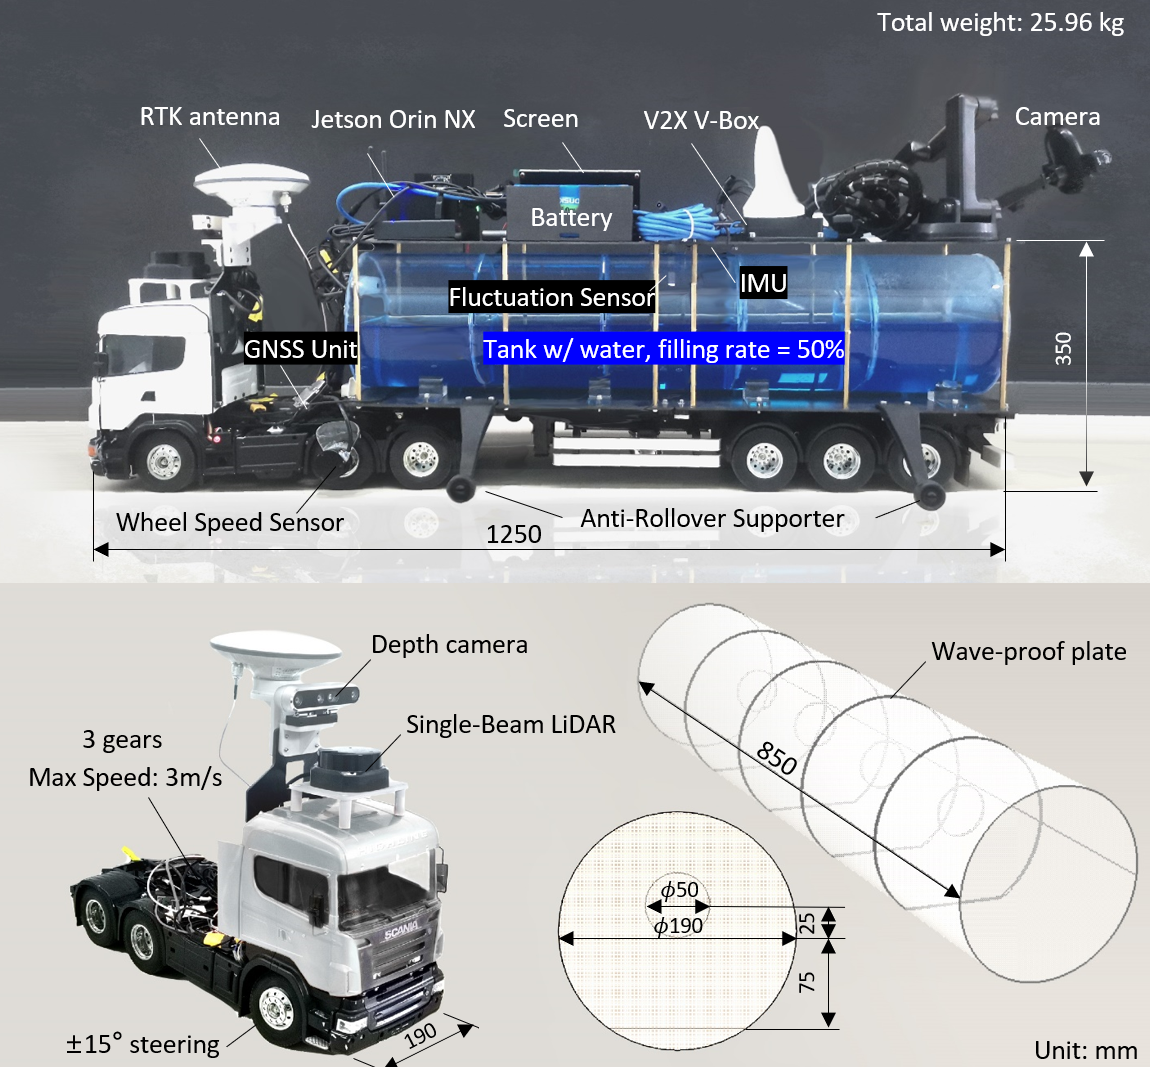
\includegraphics[width=0.32\textwidth]{fig/mod_truck.png}
    \label{fig:mod_truck}}
 % \hfill
  \subfloat[]{
    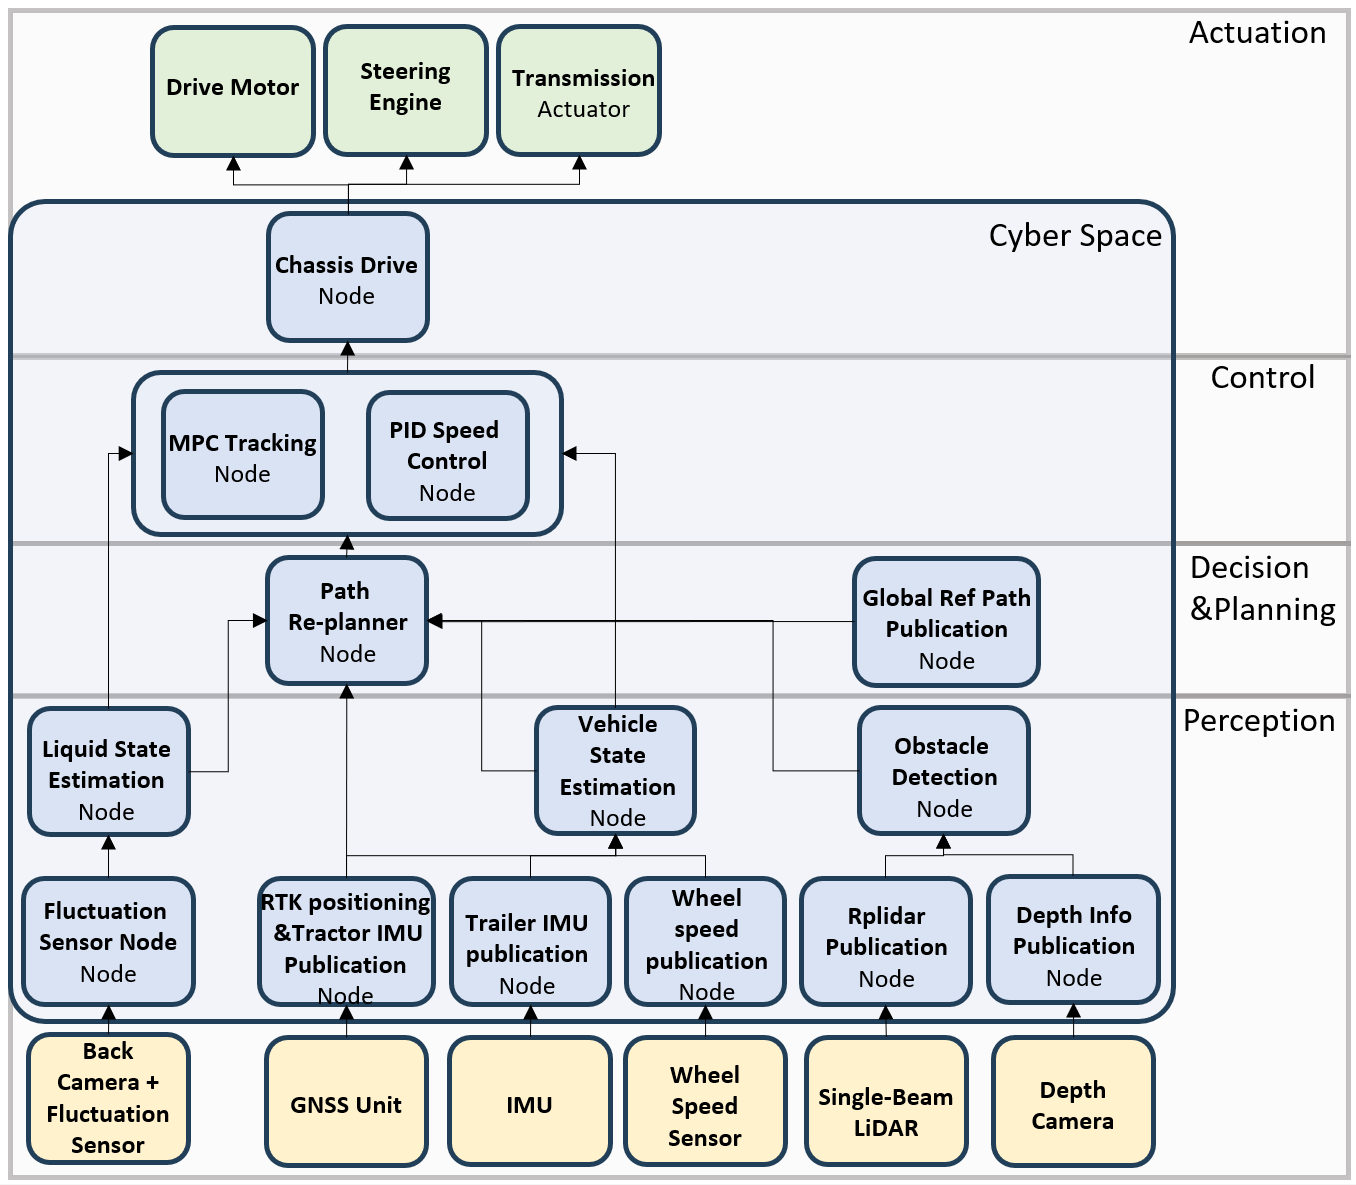
\includegraphics[width=0.34\textwidth]{fig/mod_architecture.png}
    \label{fig:mod_architecture}} 
  \subfloat[]{
    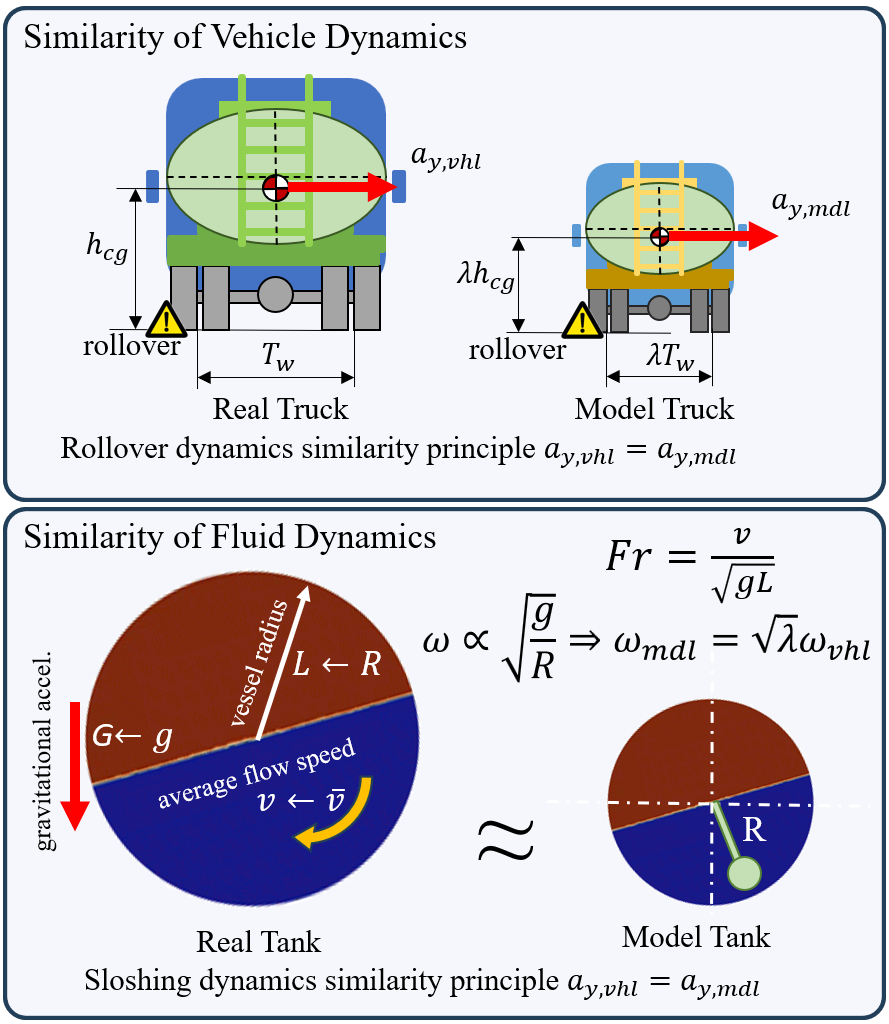
\includegraphics[width=0.26\textwidth]{fig/mod_similarity.png}
    \label{fig:mod_similarity}
  }

  \vspace{-0.3cm}
  \subfloat[]{
    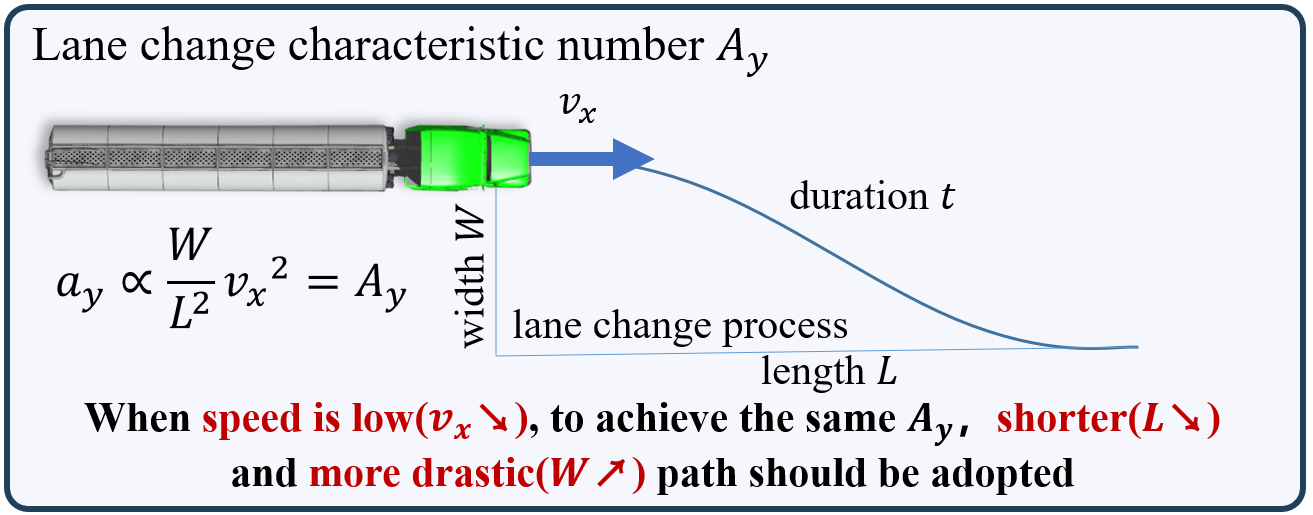
\includegraphics[width=0.35\textwidth]{fig/mod_lanechange_character.png}
    \label{fig:mod_lane_change_char}
  }
  \subfloat[]{
    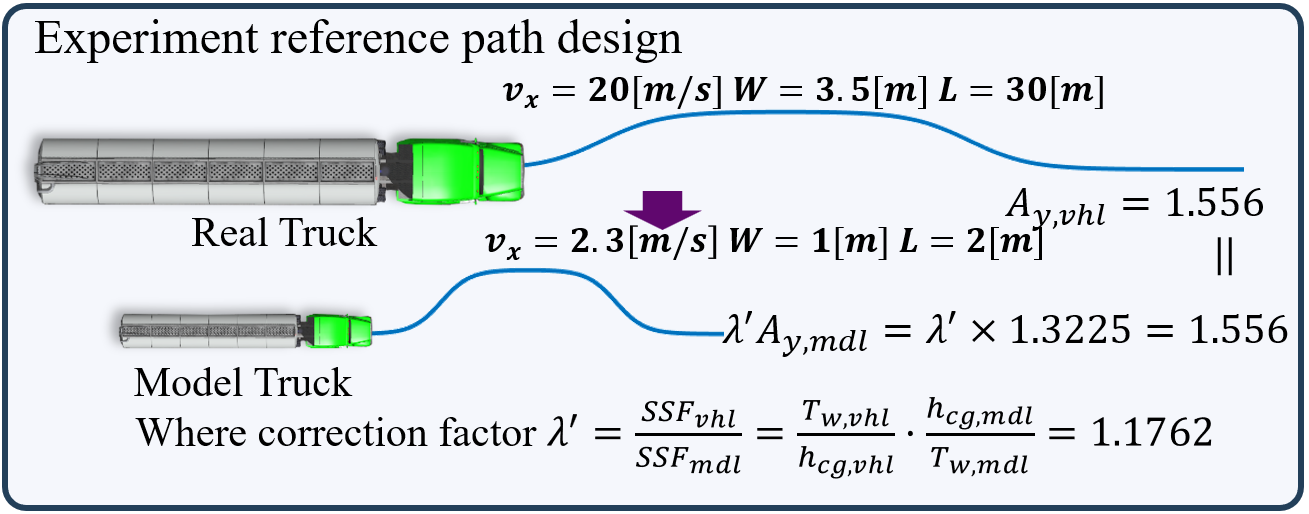
\includegraphics[width=0.33\textwidth]{fig/mod_exp_path_design.png}
    \label{fig:mod_path}
  }
  
  \caption{Model semi-trailer tank truck experimental platform, similarity principle and path design. (a)Hardware layout of model truck. (b)Program architecture realizing experiment functions. (c)Vehicle and fluid dynamics similarity principle. (d)Lane change characteristic number. (e)Reference path design for experiment.}
  \label{fig:model_truck}
  \vspace{-0.5cm}
\end{figure*}

\subsubsection{Model truck platform}
As shown in Fig. \ref{fig:mod_truck}, the main body of the model semi-tanker truck is a high-precision 1:14 TAMIYA semi-truck model with size 1250mm (L) x 200mm (W) x 400mm (H). The overall dimensions remain the same regardless of whether a liquid tank is installed. Size of liquid tank model is 850mm (L) x 190mm (W) x 190mm (H). The total weight of the model is 25.96kg, and its maximum speed is approximately 3m/s. It is equipped with anti-rollover supports that can withstand vehicle tilting up to 15° to prevent actual rollovers of the model.

The sensor configuration includes a Slamtec-S2 LiDAR, an Intel-D455 depth camera for environmental perception, an FDLink nine-axis GNSS combined with trailer IMU for vehicle pose estimation, a WHEELTEC rotary encoder as a wheel speed sensor and another modified as a fluctuation sensor, and a rear camera for recording liquid motion. The domain controller utilizes the Jetson Orin NX (16GB RAM, 100TOPS). State variables are available through measurement in Table.\ref{tab:measurement}.

\vspace{-0.5cm}
\begin{table}[!htbp]
  \centering
  \caption{Means of Measurement for State Variables}
  \vspace{-0.2cm}
  \label{tab:measurement}
  \begin{tabularx}{0.45\textwidth}{@{}lX@{}}
    \toprule
    \textbf{State} & \textbf{Means of measurement} \\
    \midrule
    $v_{1y}\,v_{2y}$ & estimation based on Kalman Filter\cite{FengRan2018}\\
    $\dot{\psi}_1\,\phi_1\,\dot{\phi}_1$ & FDLink nine-axis GNSS(IMU + RTK) \\
    $\dot{\psi}_2\,\phi_2\,\dot{\phi}_2$ & FDLink nine-axis IMU \\
    $\theta\,\dot{\theta}$ & WHEELTEC rotary encoder(as fluctuation sensor in tank)\\
    $Y_1\,X_1\,\psi_1$ & FDLink nine-axis GNSS(IMU + RTK) \\
    $v_{1x}$ & WHEELTEC rotary encoder(as wheel speed sensor) \\
    \bottomrule
  \end{tabularx}
  \vspace{-0.3cm}
\end{table}


The liquid tank is made of acrylic material with a thickness of 3mm and features interval-configured anti-surge plates, simulating the commonly seen circular tanks with anti-surge plates in real-world scenarios \cite{WanYing2018}. This model provides an integrated experimental platform that closely mimics real-world conditions for validating anti-rollover control algorithms for liquid tankers.

\subsubsection{Program architecture}
The vehicle implements anti-rollover path tracking functionality through the program architecture shown in Fig. \ref{fig:mod_architecture}. The perception layer provides liquid state estimation and target-level perception information using a rear camera for capturing liquid motion. The decision-making and planning layer includes a pre-defined global reference path and a path re-planner. The control layer consists of MPC-based lateral control for anti-rollover path tracking and a PID controller for longitudinal control. The algorithms run on ROS in Ubuntu 20.04, with the MPC algorithm implemented in C++ for real-time performance and other nodes implemented in Python.


















\vspace{-0.5cm}
\subsection{Similarity Principle of Model Experiment}

Similarity is a necessary condition for using a model to replace a prototype in experiments. For the same physical process, if the corresponding physical quantities of two phenomena are proportional at each corresponding point and moment, and the corresponding directions of the vectors are consistent, then these two phenomena are considered similar \cite{BookFluidMechanics}. To use a model vehicle to validate the control effectiveness under extreme conditions instead of a real vehicle, it is necessary to ensure similarity in both vehicle dynamics and fluid dynamics.

In this study, vehicle dynamics similarity refers to rollover dynamics similarity, which can be quantitatively characterized by the static stability factor (SSF). As shown in Fig. \ref{fig:mod_similarity}, if all geometric parameters and mass distributions of the model are scaled by a proportionality factor $\lambda > 0$, and the SSF of the real vehicle and the model are the same, then the real vehicle and the model vehicle will experience rollover only when they have the same lateral acceleration, i.e.


\vspace{-0.3cm}
\begin{equation}
a_{y,vhl} = a_{y,mdl}
\end{equation}

However, due to limitations, it is difficult for actual model to meet the conditions of proportional scaling, so a correction coefficient $
\lambda^{'}$ needs to be introduced

\vspace{-0.3cm}
\begin{equation}
\lambda^{'} = \frac{SSF_{vhl}}{SSF_{mdl}} = \frac{T_{w,vhl}}{h_{cg,vhl}} \cdot \frac{h_{cg,mdl}}{T_{w,mdl}}
\end{equation}

i.e. experiment is similar when equation(\ref{eq:similarity}) is satisfied

\vspace{-0.3cm}
\begin{equation}
a_{y,vhl} = \lambda^{'}a_{y,mdl}
\label{eq:similarity}
\end{equation}

For fluid with free surface, the flow is mainly governed by inertial forces. Therefore, the Froude number $Fr$ is used as a similarity criterion, where $Fr = \frac{v}{\sqrt{gL}}$. Here, $v$ represents the characteristic velocity of the fluid, typically the average flow velocity $\bar{v}$; $g$ represents the gravitational acceleration, and for lateral excitation, the acceleration is relatively small, so we can consider $G=g$. In the small amplitude linear sloshing inside the tank, the liquid can be approximated as a pendulum, with its length approximate to tank radius $R$. The sloshing frequency $\omega$ decreases as $R$ increases, following the relationship

\vspace{-0.3cm}
\begin{equation}
\left. \omega \propto \sqrt{\frac{g}{R}}\Rightarrow\omega_{mdl} = \sqrt{\lambda}\omega_{vhl} \right.
\end{equation}

In relationship above, can be found that for sloshing in tanks, as long as the lateral acceleration difference is not too large, the resultant acceleration approximates to $g$. Therefore, in both the actual tank and the model tank, $Fr$ of liquid can be considered equal,

\vspace{-0.5cm}
\begin{equation}
\begin{split}
Fr_{mdl} &= \frac{v_{mdl}}{\sqrt{G_{mdl}L_{mdl}}} = \frac{\omega_{mdl}R_{mdl}}{\sqrt{gR_{mdl}}} 
= \omega_{mdl}\sqrt{\frac{R_{mdl}}{g}}\\ &= \sqrt{\lambda}\omega_{vhl}\sqrt{\frac{R_{vhl}}{\lambda}} = \omega_{vhl}\sqrt{\frac{R_{vhl}}{g}} \approx Fr_{vhl}
\end{split}
\end{equation}

In summary, as long as the lateral acceleration relationship in equation(\ref{eq:similarity}) is met, the lateral rollover dynamics and liquid sloshing characteristics of the model semi-trailer tank truck can be considered similar to the prototype.


\vspace{-0.5cm}
\subsection{Experiment Scenario and Results}

Due to the inclusion of single lane change, which represents a more representative scenario, the double lane change maneuver was selected for experimental validation. Based on the principle of similarity, the DLC reference path is designed (Fig. \ref{fig:mod_path}). Assuming duration of lane change one is $t$, with the length $L$ and width $W$, it can be considered that lateral velocity $
v_{y} \propto W/t$, while $t\propto L/v_x$. The lateral acceleration $
a_{y} \propto \Delta v_{y}/t \propto v_{y}/t$. We define the lane change characteristic number as equation(\ref{eq:lane_change_char}), Fig. \ref{fig:mod_lane_change_char}. 

\vspace{-0.3cm}
\begin{equation}
A_{y} = \frac{W}{L^{2}}{v_{x}}^{2} \propto a_{y}
\label{eq:lane_change_char}
\end{equation}


\begin{figure*}[htbp]
  \centering
  \begin{minipage}{0.30\textwidth}
    \centering
    \subfloat[]{
      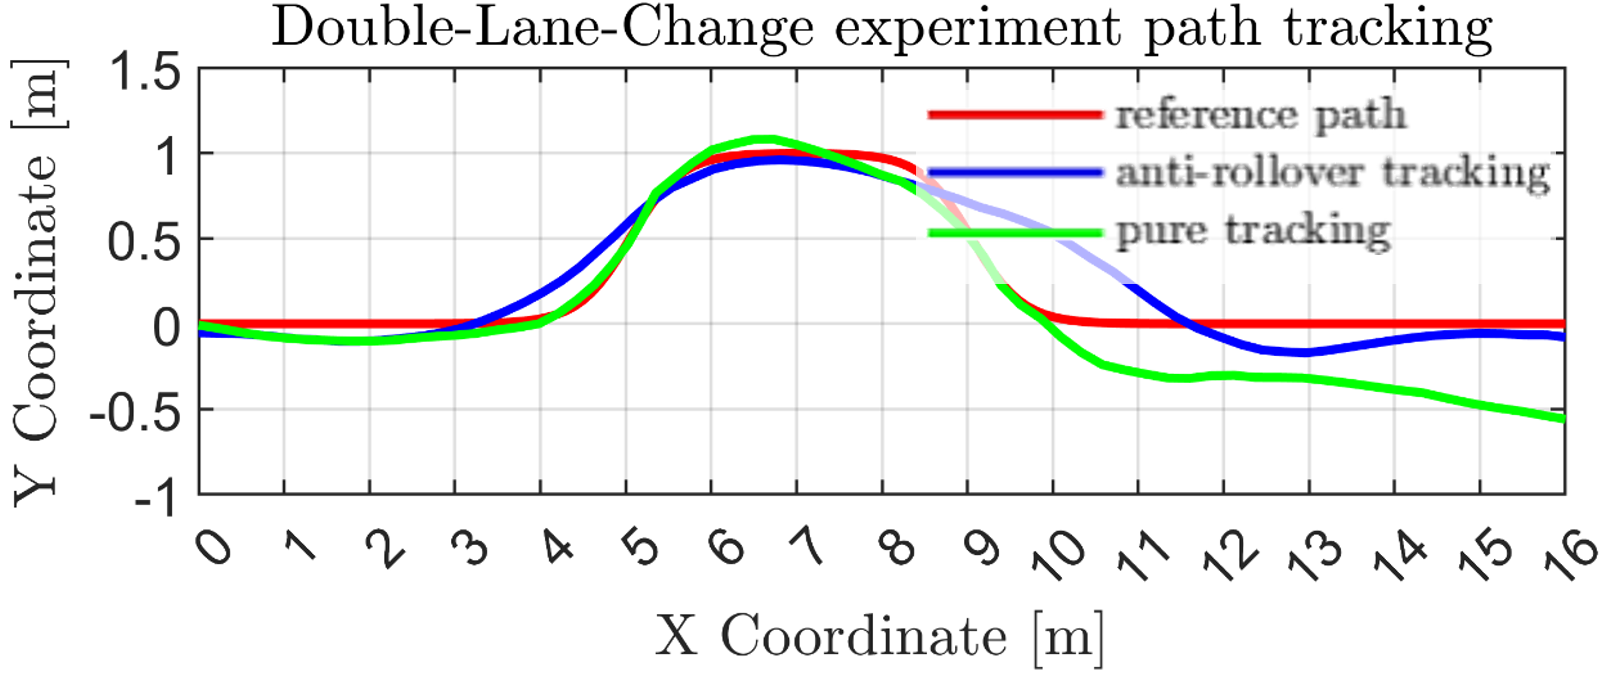
\includegraphics[width=\textwidth]{fig/exp_tracking.png}
      \label{fig:exp_tracking}\vspace{-0.3cm}}\vspace{-0.4cm}
    
    \subfloat[]{
      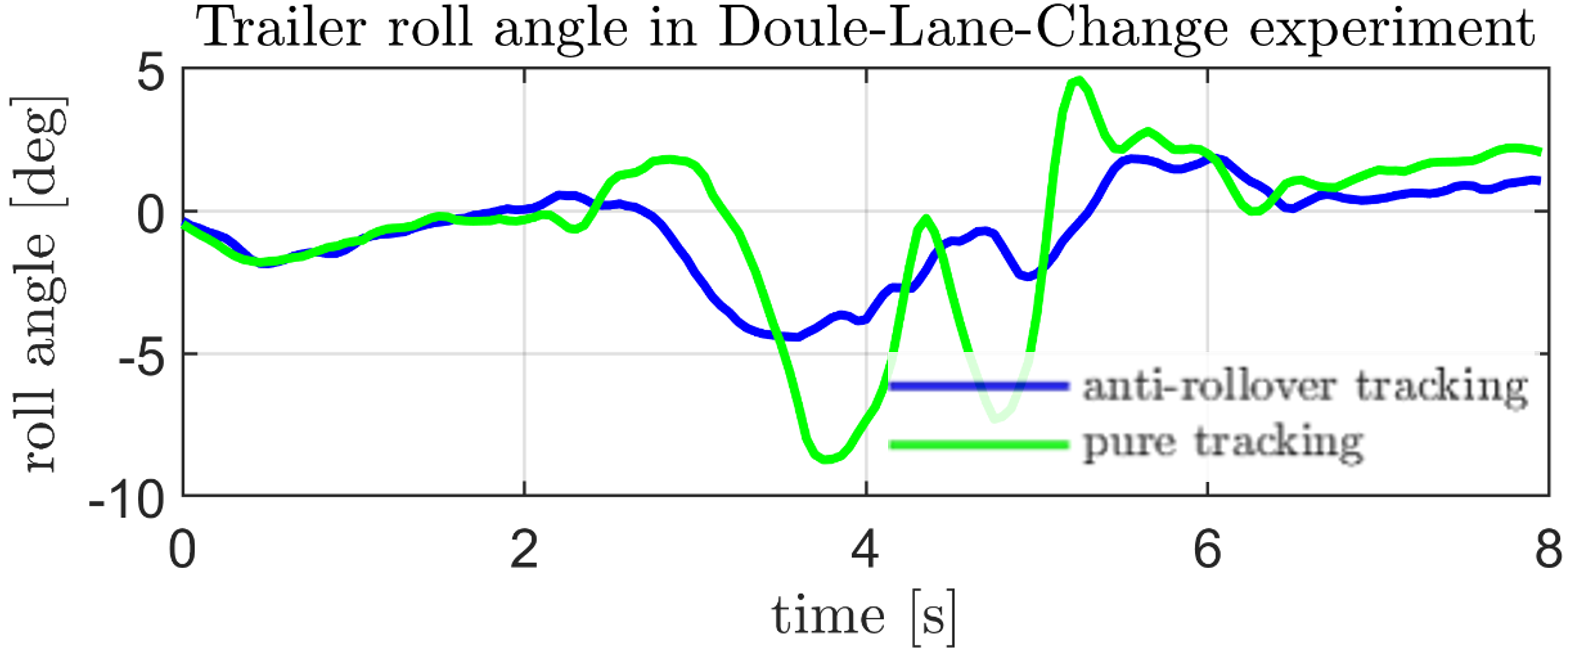
\includegraphics[width=\textwidth]{fig/exp_roll.png}
      \label{fig:exp_roll}\vspace{-0.3cm}}\vspace{-0.4cm}
    
    \subfloat[]{
      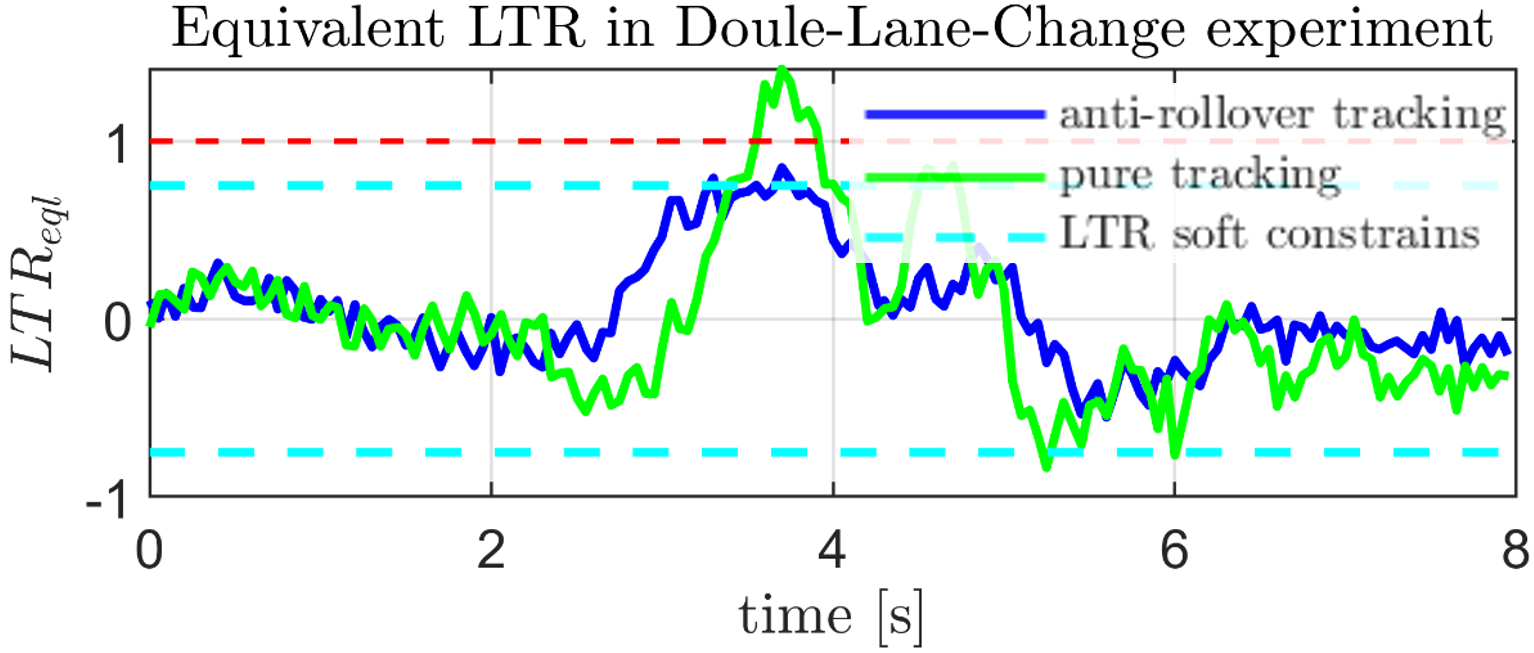
\includegraphics[width=\textwidth]{fig/exp_LTR.png}
      \label{fig:exp_LTR}\vspace{-0.3cm}}
  \end{minipage}
  \begin{minipage}{0.33\textwidth}
    \centering
    \subfloat[]{
      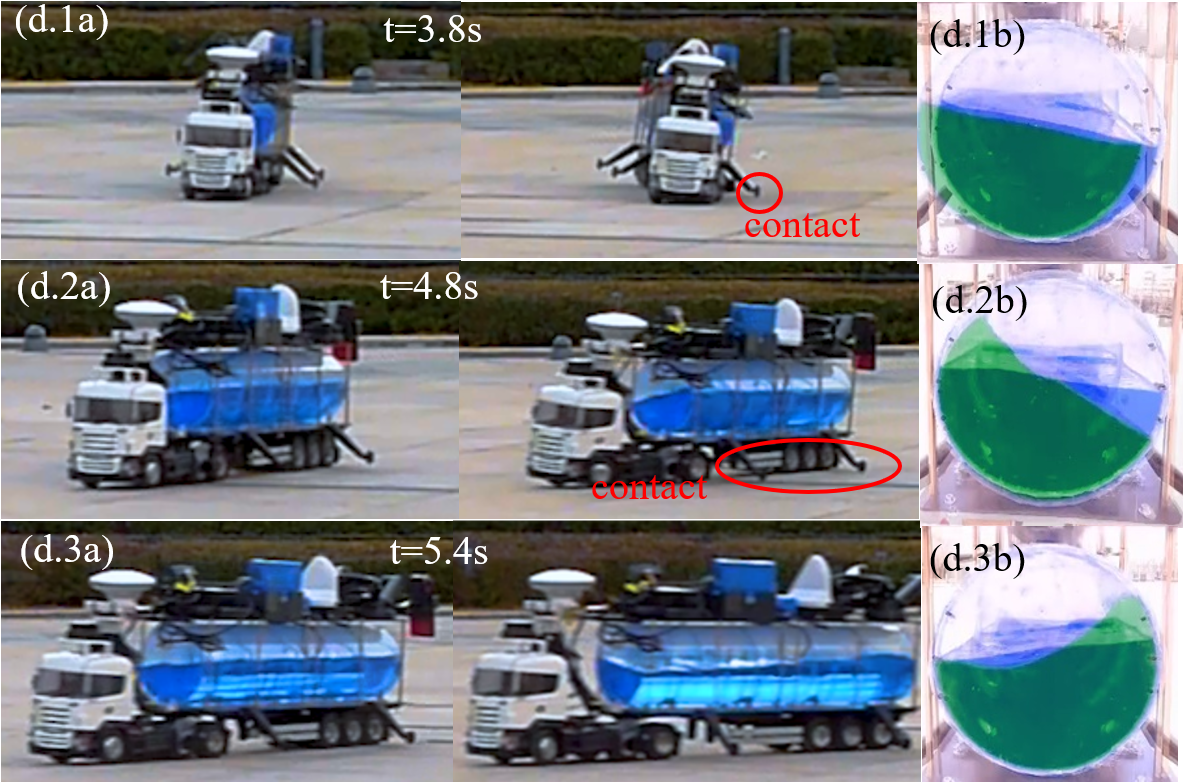
\includegraphics[width=\textwidth]{fig/exp_photos.png}
      \label{fig:exp_photos}}\vspace{-0.3cm}
    
    \subfloat[]{
      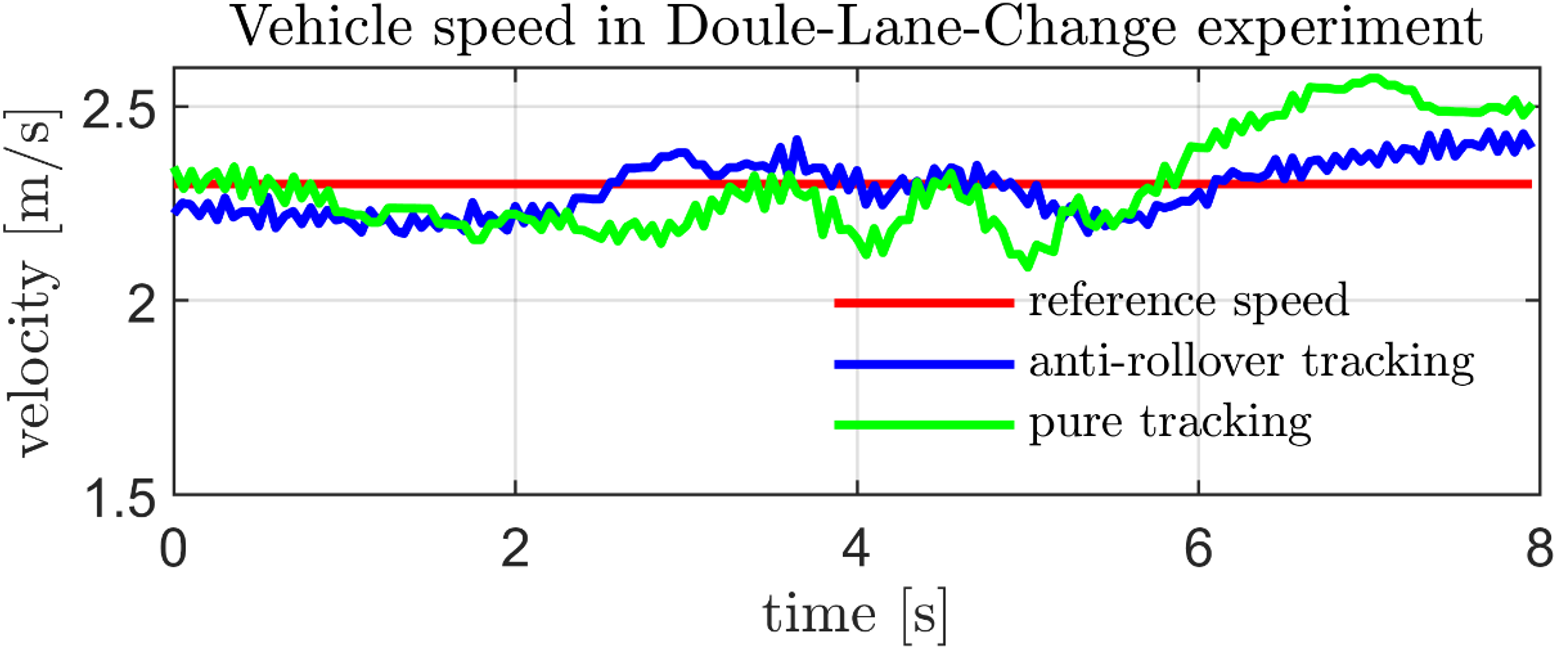
\includegraphics[width=\textwidth]{fig/exp_vel.png}
      \label{fig:exp_vel}}
  \end{minipage}
  \begin{minipage}{0.33\textwidth}
    \centering
    \subfloat[]{
      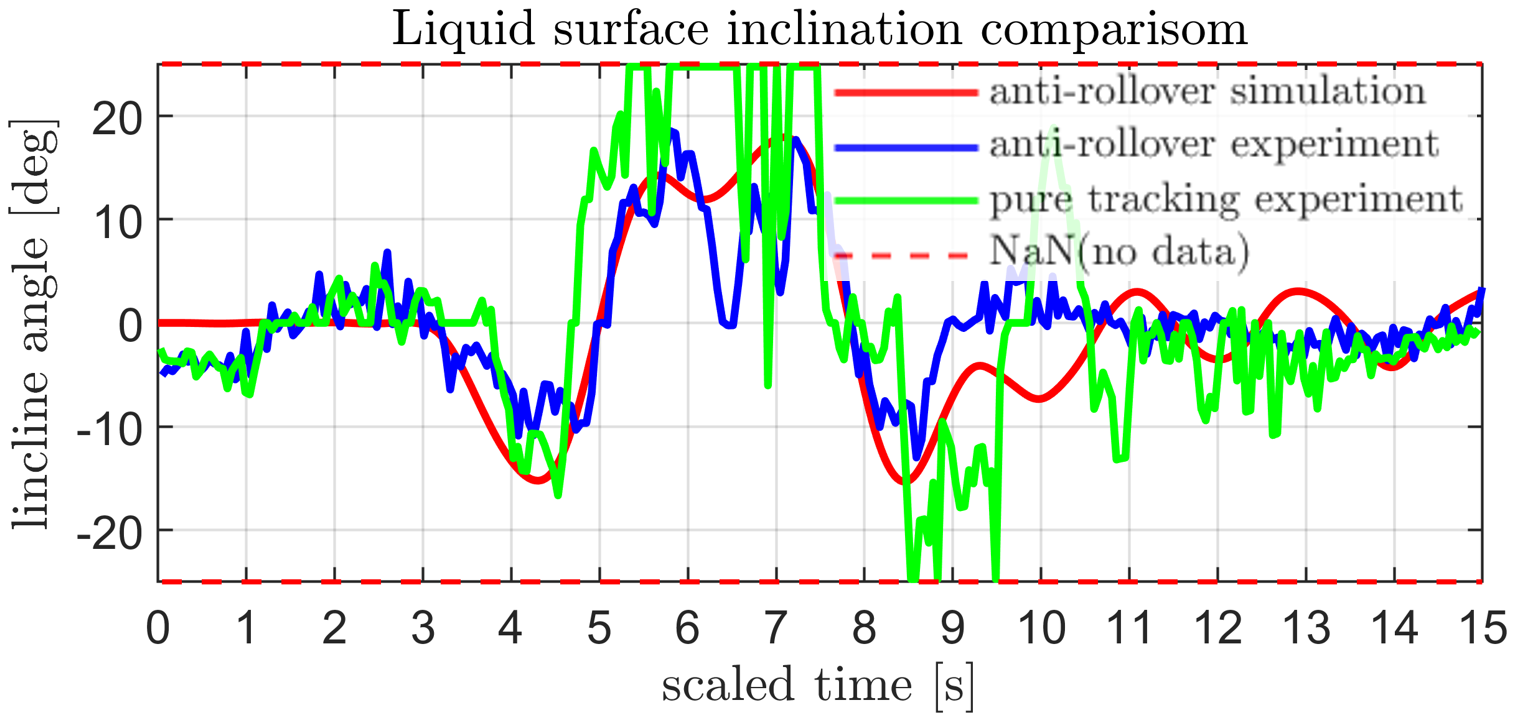
\includegraphics[width=\textwidth]{fig/exp_sloshing_angle.png}
      \label{fig:exp_sloshing}}\vspace{-0.3cm}
    
    \subfloat[]{
      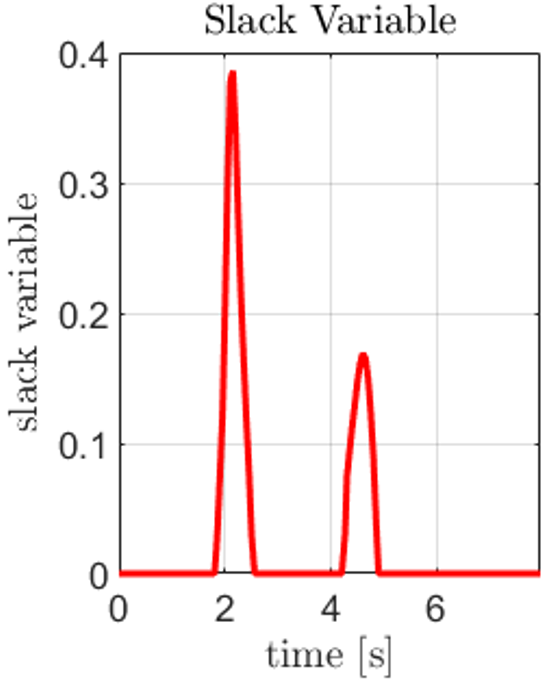
\includegraphics[width=0.45\textwidth]{fig/exp_slackVar.png}
      \label{fig:exp_slk}}\hspace{-0.1cm}
    \subfloat[]{
      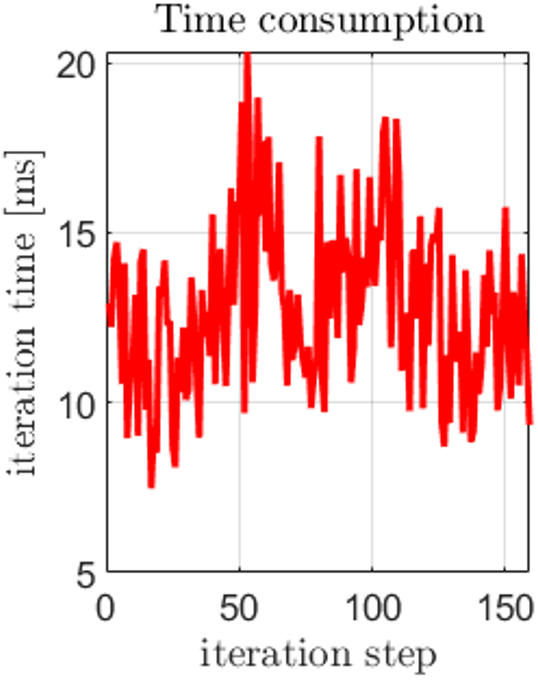
\includegraphics[width=0.45\textwidth]{fig/exp_iterTime.png}
      \label{fig:exp_iterTime}}\vspace{-0.3cm}
  \end{minipage}
  \vspace{-0.3cm}
  \caption{Truck experiment results. (a)Tracking performance. (b)Roll status comparison of trailer. (c)$LTR_{eql}$ comparison. (d)Experiment snapshots in key time points (d.$i$a, left: anti-rollover group, right: preview tracking group. d.$i$b, green: anti-rollover group, blue: preview tracking group. $i = 1, 2, 3$). (e)Velocity in double lane change. (f)Liquid sloshing angle comparison. (g) Slack variable value. (h)Algorithm time consumption in each control cycle.}
  \label{fig:experiment}
  \vspace{-0.7cm}
\end{figure*}





For the experiment, we used the same parameters of controller frequency 20 $Hz$, $N_p = 40$, $N_c = 3$, and $N_r = 20$ as in the simulation. Experimental results, as shown in Fig.\ref{fig:experiment}, compare anti-rollover control with preview tracking. Both groups maintained a speed of approximately 2.3 $m/s$ (Fig.\ref{fig:exp_vel}). In Fig.\ref{fig:exp_tracking}, the anti-rollover group performed an early lane change and delayed the return, keeping $LTR_{eql}$ within the soft constraints to ensure path tracking without rollover. The anti-rollover group kept the trailer roll angle within $\pm 5\degree$, with a maximum liquid surface tilt angle of approximately $20\degree$. The preview tracking group focused solely on path tracking, resulting in small tracking errors but excessive lateral acceleration causing severe liquid sloshing. Although the presence of anti-rollover support prevented actual rollover, Fig.\ref{fig:exp_photos} shows that the anti-roll supporter touched the ground at $t=3.8s$ and $t=4.8s$. In a real vehicle, this would correspond to a rollover event. After the double lane change segment, the intense vehicle body oscillation made it difficult for the preview tracking group to continue accurately, resulting in significant deviations. In contrast, the anti-rollover group remained relatively stable throughout the entire double lane change process and quickly recovered normal tracking performance. The preview tracking group exhibited trailer roll angles of approximately $9\degree$ and $7\degree$ at the end of the first and beginning of the second lane changes, respectively, namely a maximum 42\% reduction in roll angle. $LTR_{eql}$ exceeded 1 at 3.5s, indicating a potential rollover. With the support of the anti-rollover frame, $LTR_{eql}$ experienced a rebound from 3.7s to 4.3s, but the anti-roll supporter touched the ground again during the return maneuver. The preview tracking group exhibited severe liquid sloshing and showed significant nonlinearity. In Fig.\ref{fig:exp_sloshing}, there were multiple instances where the liquid surface tilt angle could not be identified, while the anti-rollover group maintains sloshing angle within -20$\degree$-20$\degree$. The violent liquid sloshing was one of the main causes of rollover.

Fig.\ref{fig:exp_sloshing} rescales the experimentally obtained liquid surface tilt angle along the time axis by a factor of $(L_{vhl}/v_{vhl})/(L_{mdl}/v_{mdl})=1.725$. The curves of the model preview tracking group and the simulation preview tracking group have consistent amplitude and phase heights, further validating the effectiveness of the model experiments and similarity criteria.

As shown in Fig.\ref{fig:exp_iterTime}, the proposed anti-rollover path tracking algorithm has an average solution time of 13.2 $ms$ and a peak solution time of less than 20 ms, making it suitable for practical applications.













